La interfaz de lectura ASD\cite{1999ATLASICs} es un sistema de 16 canales utilizado para la lectura de detectores TGC en la Big Wheel del experimento ATLAS, como se mencionó en la sección \ref{sec:atlas}. El principal proposito de esta interfaz es detectar pulsos de alta frecuencia provenientes de detectores TGC, los cuales forman parte del Level-1 Trigger en el Espectrómetro de muones. Cada canal se corresponde con un strip o cable de un detector, por lo que al analizar las señales de salida de esta tarjeta permite determinar los vértices de interaccion de muones con el detector.

La Figura \ref{img:asd-board} corresponde a una fotografía de esta interfaz, destacando sus conectores principales y sus canales de entrada. Los canales son llamados \textit{Hits} y se enumeran del 0 al 15. Posee un conector de 40 pines para cable plano para conexión a su fuente de voltaje, para la transmisión de las señales de salida y para el ingreso de pulsos de prueba. El detalle de cada pin se ilustra en la Figura \ref{img:asd-ports}

\begin{figure}[h]
	\centering
	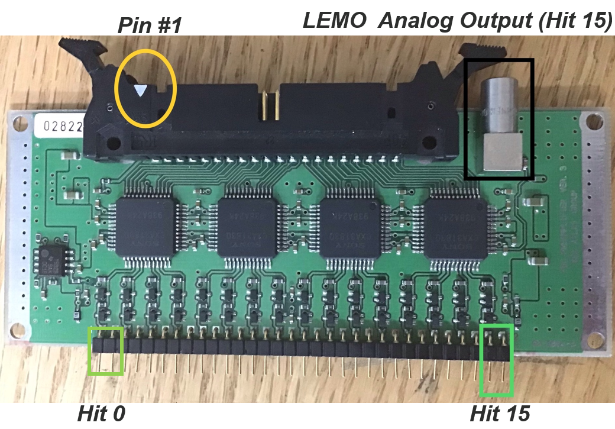
\includegraphics[scale=0.55]{asd-board.png}
	\caption{Interfaz de lectura ASD. Se destacan en la imagen sus canales (hit) del 0 al 15, su salida analógica LEMO y el primer pin en su conector de 40 posiciones.}
	\label{img:asd-board}
\end{figure}

\begin{figure}[h]
	\centering
	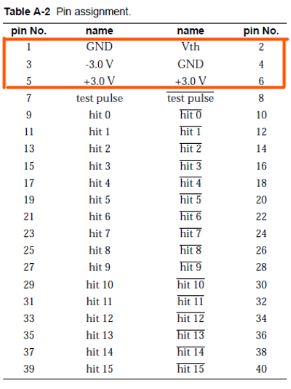
\includegraphics[scale=1]{asd-ports.png}
	\caption{Detalle de los puertos en el conector 40 posiciones de la interfaz ASD.}
	\label{img:asd-ports}
\end{figure}

Como su acrónimo lo indica, la interfaz ASD (Amplificator-Shaper-Discriminator) \jgnote{Decidi introducir de nuevo esta sigla, a pesar de que ya la defini anteriormente en la seccion \ref{sec:atlas}} amplifica la carga eléctrica captada desde un canal de un detector; modifica la forma del pulso eléctrico en cuanto a su tiempo de duración y a su amplitud de corriente con el fin de simplificar su posterior medición; y discrimina la amplitud del pulso mediante un circuito comparador. Esta comparación se realiza respecto a un nivel de voltaje ajustable para así descartar eventos de energía que estén por debajo el umbral de interés, y también para generar una señal de salida digital LVDS (Low-Voltage Differential signal) cuya duración sea proporcional a la amplitud de pulso que ha estado por sobre el umbral de voltaje configurado. Esta técnica se conoce como TOT y es la mísma técnica utilizada en el detector LabPet II descrito en la sección \ref{par:labpet}.  En la Figura \ref{fig:sistema-completo}, este pulso digital se representa como el pulso digital azul entre la interfaz de lectura y el sistema de adquisición de datos.
        
La interfaz ASD será utilizada conectándola a los strips de los detectores sTGC fabricados para sTGC Minería. Dado que la interfaz posee 16 canales de entrada, es posible conectar los 16 canales de detección proveniente de un mismo detector prototipo sTGC. Así, con un solo detector y una interfaz es posible determinar vértices de interacción en un área de 15cm$^2$. Para un futuro escalamiento, utilizando dos detectores superpuestos y sus respectivas interfaces es posible determinar la trayectoria de los muones detectados. Además, analizar la duración de cada pulso emitido por las interfaces permite estimar la amplitud de la carga eléctrica depositada por el muon en el detector excitado.


\subsection{Circuito}
La interfaz de lectura ASD tiene 16 canales que reciben impulsos de carga eléctrica provenientes de strips o cables de detectores TGC, y emite señales digitales representando estos pulsos en formato LVDS según la norma IEEE LVDS Standard 1596.3-1996\cite{1996IEEESociety}.

Esta interfaz requiere una fuente de voltaje de -+3V\cite{1999ATLASICs}, es capaz de recibir pulsos ente -1.2pC a +2.0pC sin saturarse y posee una frecuencia de entrada recomendada de hasta 100KHz. La interfaz Cuenta con un una entrada para pulsos de pruebas y una señal analógica de monitoreo proveniente de la etapa de preamplificación del canal 15, implementada con un conector LEMO.

En la Figura \ref{img:asd-circuit} se ilustra el circuito principal incluido en cada canal de la Interfaz. Cada canal tiene su propio preamplificador, un amplificador principal y un comparador\cite{1999ATLASICs}, donde la etapa de preamplificación tiene una ganancia de 0.8V/pC y el amplificador principal tiene una ganancia de 7 veces la señal entrante. La etapa de comparación compara la señal con un nivel de voltaje externo llamado \textit{V$_{th}$}. Si el pulso entrante tiene una amplitud de voltaje superior a $\frac{V_{th}}{2}$, el comparador emite una señal LVDS con una duración equivalente al tiempo durante el cual la amplitud del pulso entrante se mantuvo por sobre $\frac{V_{th}}{2}$. V$_{th}$ puede configurarse en un rango desde -0.5V a +0.5V, resultando en un umbral real de -0.25V a +0.25V en el comparador\cite{1999ATLASICs}.

\begin{figure}[h]
	\centering
	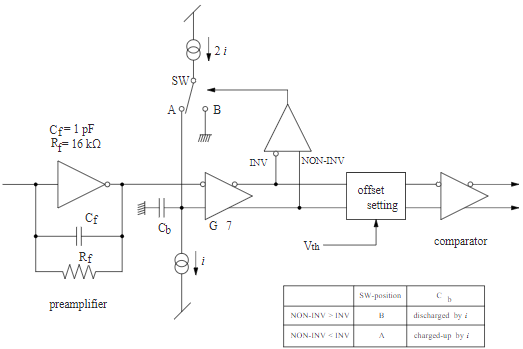
\includegraphics[scale=1]{asd-circuit.png}
	\caption{Diagrama de bloques del circuito principal para un canal de la interfaz ASD. Se indican la etapa de preamplificación, el amplificador principal de ganancia 7, y el comparador.}
	\label{img:asd-circuit}
\end{figure}

\subsection{Ejemplo de operación}

Por ejemplo, para un pulso proveniente de un cátodo (pulso de polaridad positiva) de 0.3pC, el voltaje esperado a la salida de la etapa de preamplificación es 240mV. La salida analógica LEMO podría reflejar un voltaje menor debido a la impedancia de la carga conectada para su lectura. Con una ganancia de 7 veces, el voltaje esperado a la salida del amplificador principal sería de 1,68V. La duración del pulso analógico sería aproximadamente 70ns, suponiendo un canto de subida con 10ns de duración y una carga proporcional a la carga de entrada. Con un voltaje V$_{th}$ de 180mV, la señal digital de salida tendría una duración de aproximadamente 50ns.

La Figura \ref{img:charge-injector-output} incluye un pulso de 0.3pC de carga eléctrica, mientras que la Figura \ref{img:asd-analog-output} muestra la señal analógica en el conector LEMO. La salida LEMO presenta una amplitud de 180mV, 25\% más bajo de lo esperado, probablemente debido a la impedancia de entrada del osciloscopio utilizado para su medición

\begin{figure}[h]
	\centering
	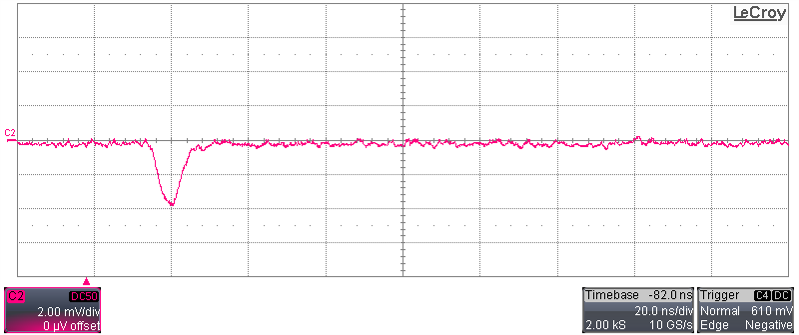
\includegraphics[scale=0.43]{charge-injector-output.png}
	\caption{Captura de pantalla de un pulso de voltaje con carga equivalente a 0.3pC, medido en un osciloscopio.}
	\label{img:charge-injector-output}
\end{figure}

\begin{figure}[h]
	\centering
	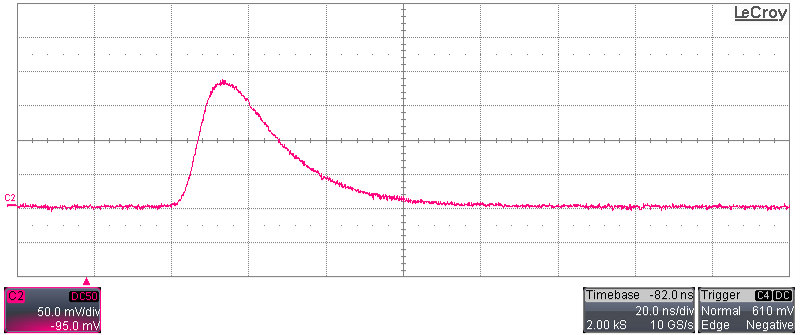
\includegraphics[scale=0.43]{asd-analog-output.png}
	\caption{Captura de pantalla de un oscilocopio, en la cual se ilustra un pulso de voltaje proveniente de la salida analógica LEMO de la interfaz ASD luego de haber recibido un pulso de 0.3pC de carga eléctrica.}
	\label{img:asd-analog-output}
\end{figure}


